\documentclass[]{article}

\usepackage[utf8]{inputenc}
\usepackage{graphicx} 
\usepackage{natbib}
\usepackage{subfiles}
\usepackage{subfigure}
\usepackage{float}
\usepackage[margin=0.7in]{geometry}
\usepackage{epstopdf}
\epstopdfsetup{update}
\usepackage{color}
\usepackage[pdfpagelabels]{hyperref}

\newcommand{\todo}[1]{\textcolor{blue}{#1}}
\newcommand{\todolist}[1]{\textcolor{blue}{\begin{itemize}#1\end{itemize}}}
\newcommand{\myNote}[2]{\textcolor{red}{#1}\footnote{\textcolor{blue}{#2}}}
\newcommand{\changed}[1]{\textcolor{blue}{#1}}

\begin{document}

\title{Model Predictive Control using Differential Dynamic Programming for Unmanned Surface Vehicle}
%\author{Author}
%\date{Today}
\maketitle

\section{Vehicle Description}

For Unmanned Surface Vehicle~(USV), we acquired the HyDrone-RCV~(\url{http://seafloorsystems.com/products/product/1-hydrone-rcv}) from Seafloor Systems. The USV is a one-man portable~(around 30Ibs without sensor), and has a wide profile to avoid tipping. Besides, its watertight design and construction helps in protecting the electronic components from water damage. It consists of two catamarans held by a metal chassis, which also act as the support for an onboard computer box for autonomous operations. It is also equipped with a WiFi for communication and a GPS for navigation. Fitted with two 12V 10ah batteries, the USV has a battery endurance of 5 $-$ 8 hours.  

\begin{figure}[h]
\centering
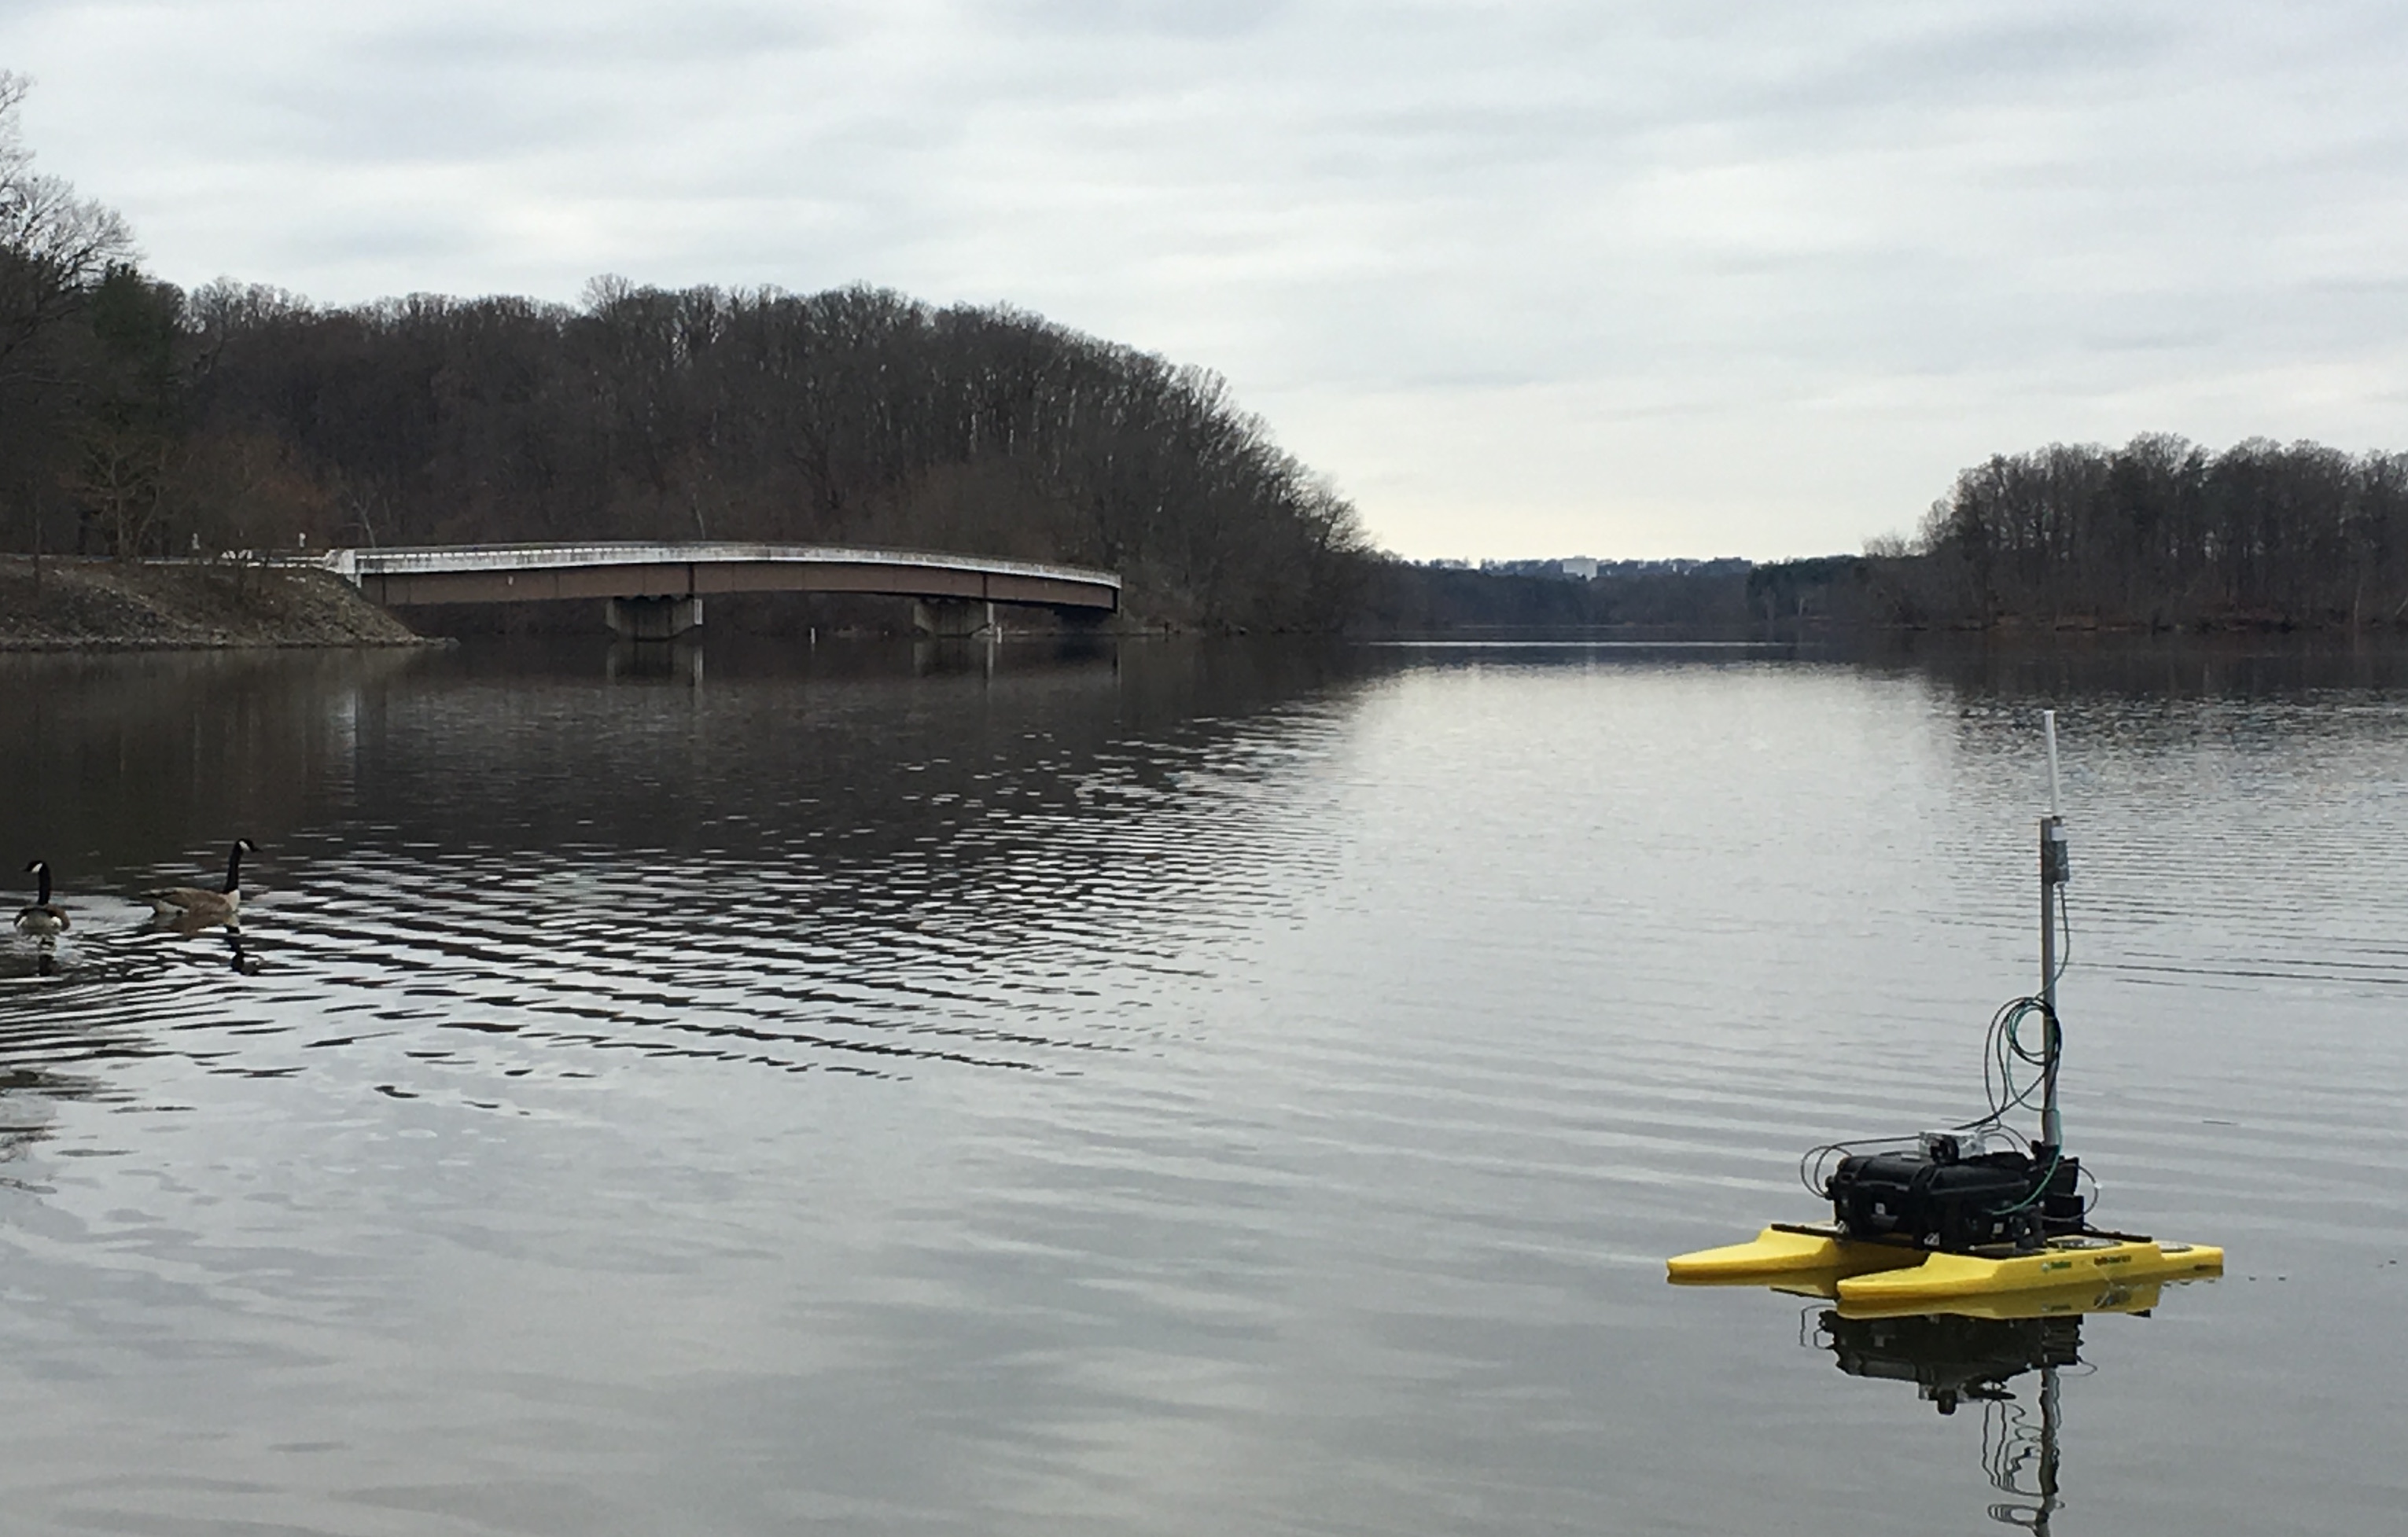
\includegraphics[width=10cm]{img/IMG_2515.JPG}
\caption{The USV operating at Loch Raven reservoir, MD.}
\label{fig:usv}
\end{figure} 



\section{System Model}

%Kinematic equation

%Dynamic equation


\section{System Identificaiton}

\subsection{Vehicle Mass and dimension}

\begin{figure}[H]
\centering
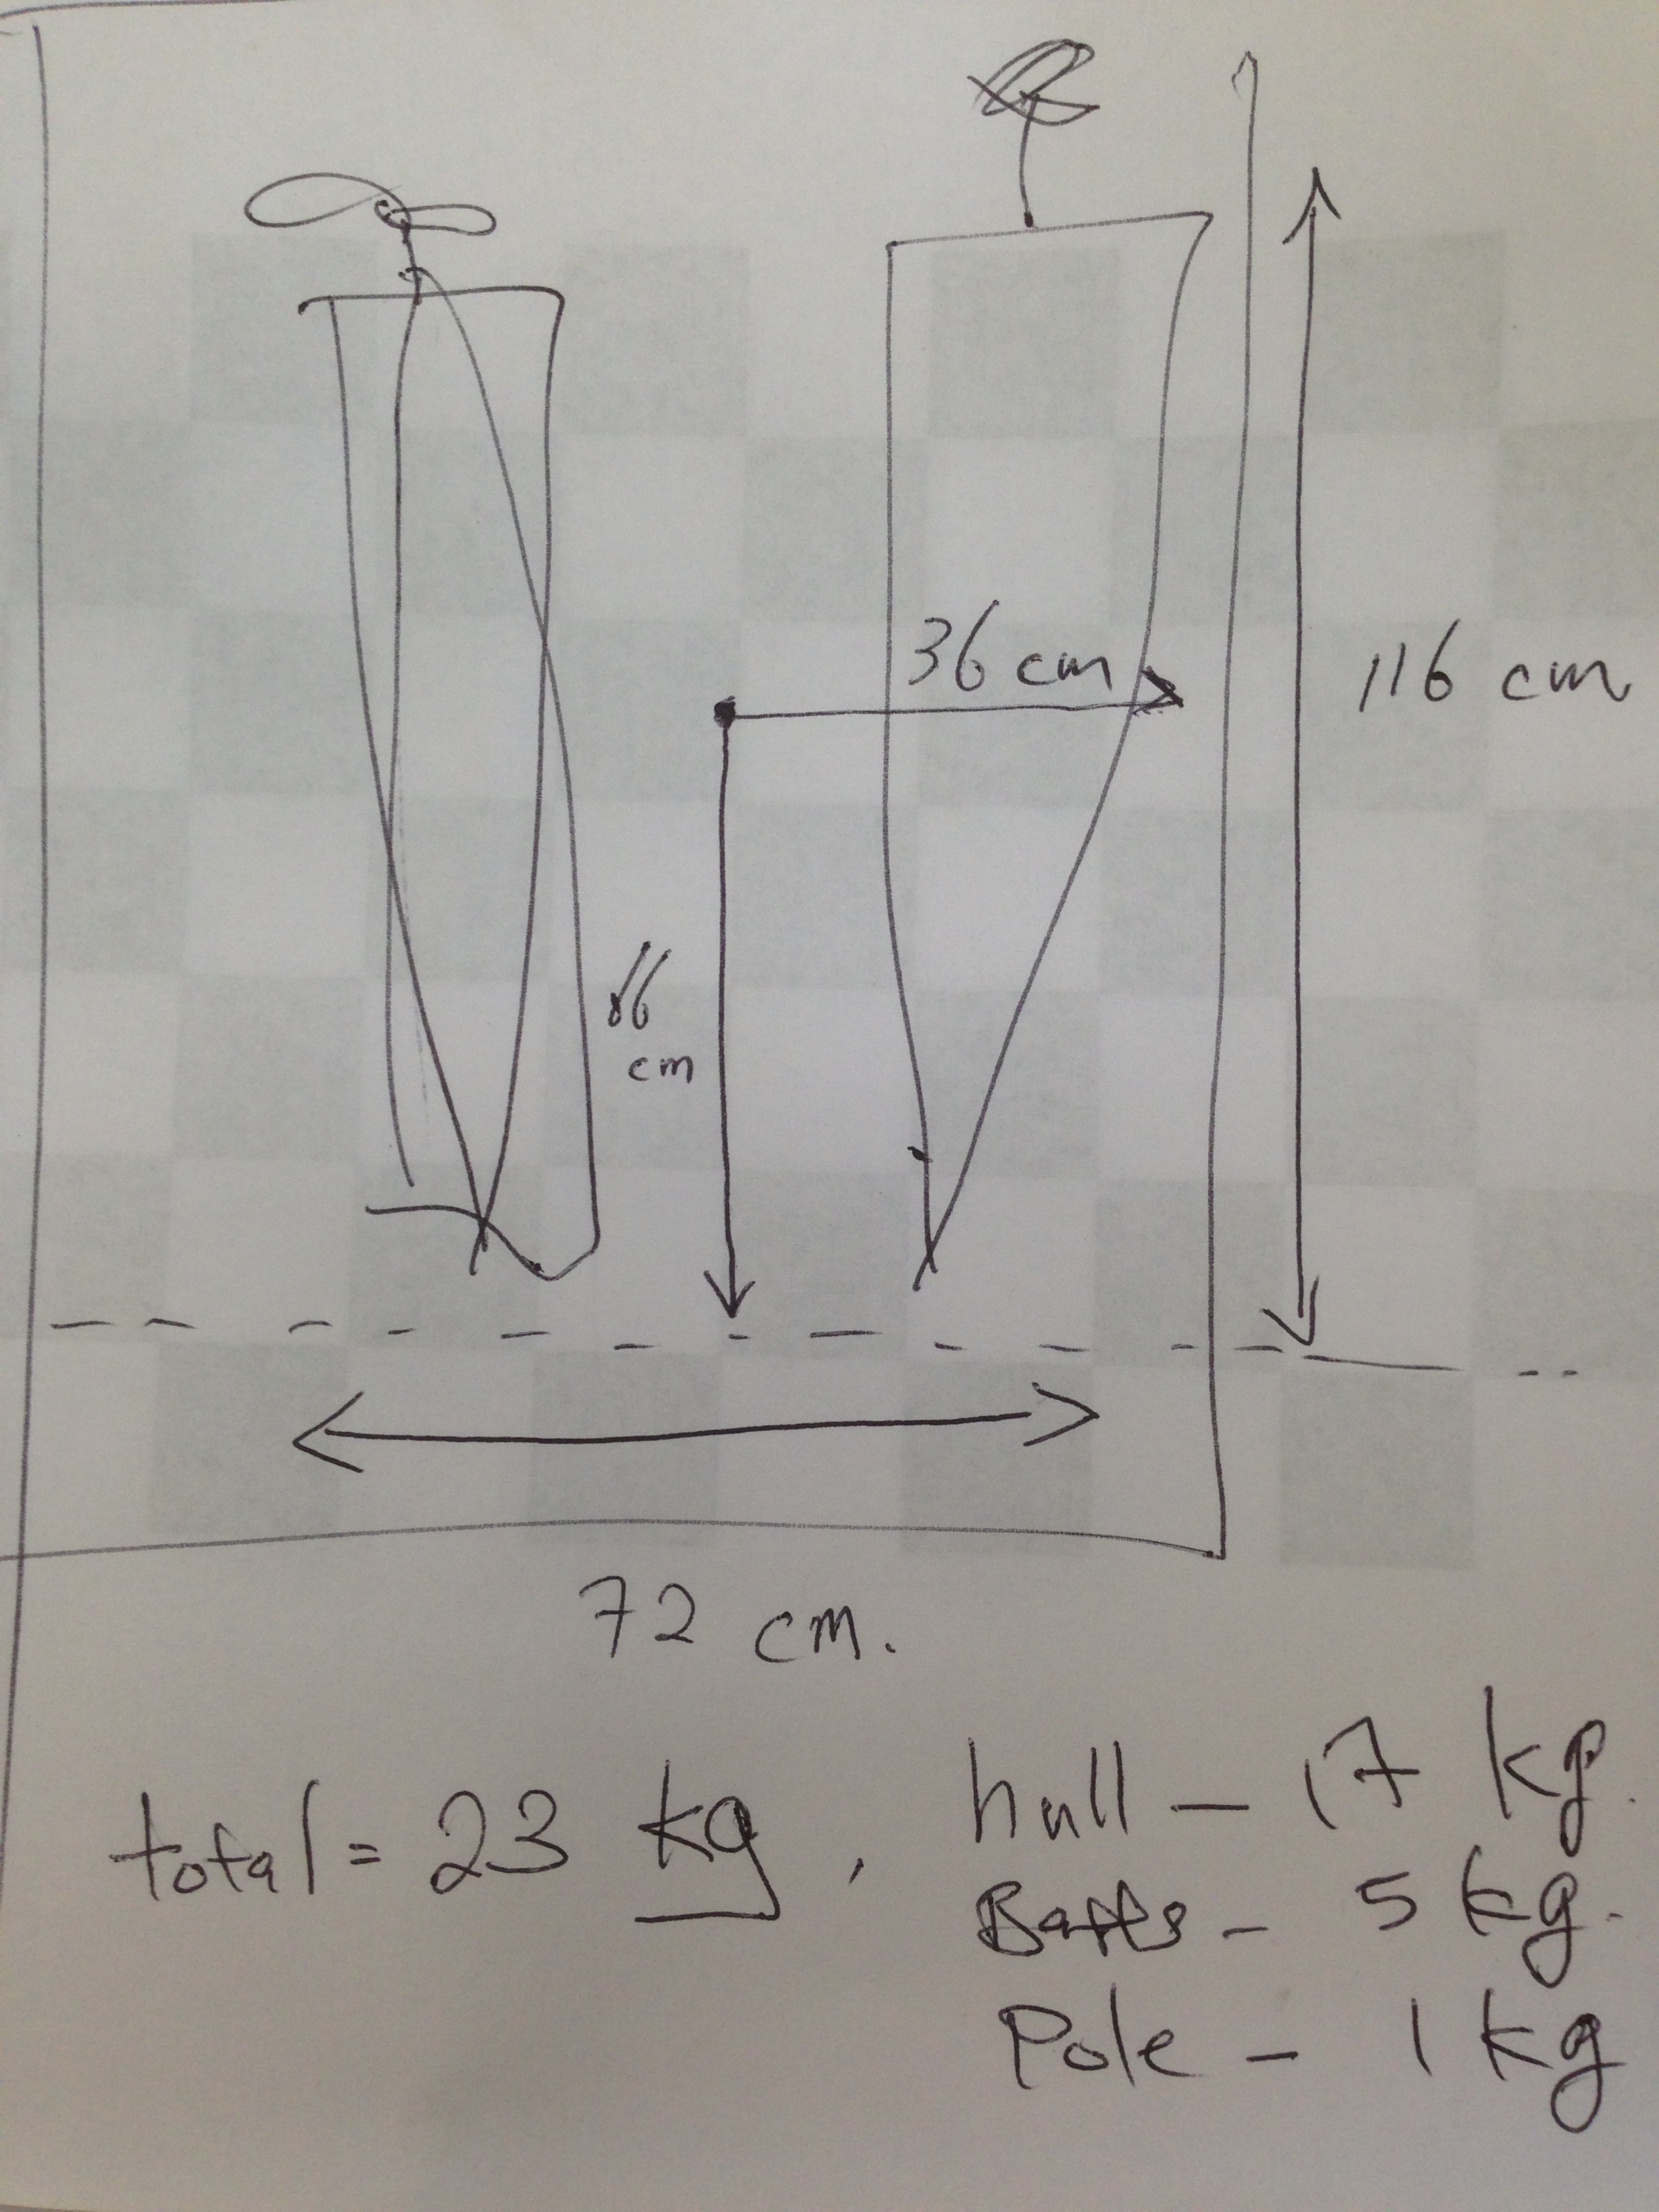
\includegraphics[width=10cm]{img/vec_dimension_mass.JPG}
\caption{The vehicle's mass and dimension.}
\label{fig:usv}
\end{figure} 

\subsection{Thruster Model Identificaiton}
The thruster model identification was performed in a tank with a force sensor and the thruster commanded to thrust at different level. However, only 0 - 50 $\%$ thrust were able to be performed, the rest were interpolated using curve fitting. 


\todo{Please insert the table of commanded thrust against measured force here !! }


\subsection{Damping Parameters Estimation}

\todo{Please briefly describe the data set used for this purpose. Plot the path used and keep the copy of dataset (only related messages) in the same folder as a backup copy}

\todo{Reference accordingly ?? \cite{Hitz01112015}}

\subsection{Performance of system ID}

\todo{A table of the parameters setup in the DDP planner. As a backup and reference}

\todo{Results from cross validation using a separate dataset}


\section{External Force Estimation}

\subsection{Simulation Results}

\todo{What is the scenario used, what is the results??}

\subsection{Field experiment}
\todo{Briefly describe the scenario and the dataset used for the estimation.}

\section{Field Experiment - Parallel Parking}

\todo{this section should include the dataset collection with closed-loop control}


\bibliographystyle{plain}
\bibliography{biblio}

\end{document}